% ============================================
% 第4章 系统详细设计与实现
% ============================================
\section{系统详细设计与实现}

本章详细阐述系统各核心模块的设计思路与实现细节，包括问卷编辑器、发布与版本管理、填写与提交、结果统计、AI 辅助和实时协作等模块。

\subsection{问卷编辑器模块}

\subsubsection{编辑器整体架构}

问卷编辑器采用三栏布局设计：左侧为题型面板，中间为编辑画布，右侧为属性设置面板。\figref{fig:editor-layout} 展示了编辑器的界面布局。

\begin{figure}[H]
\centering
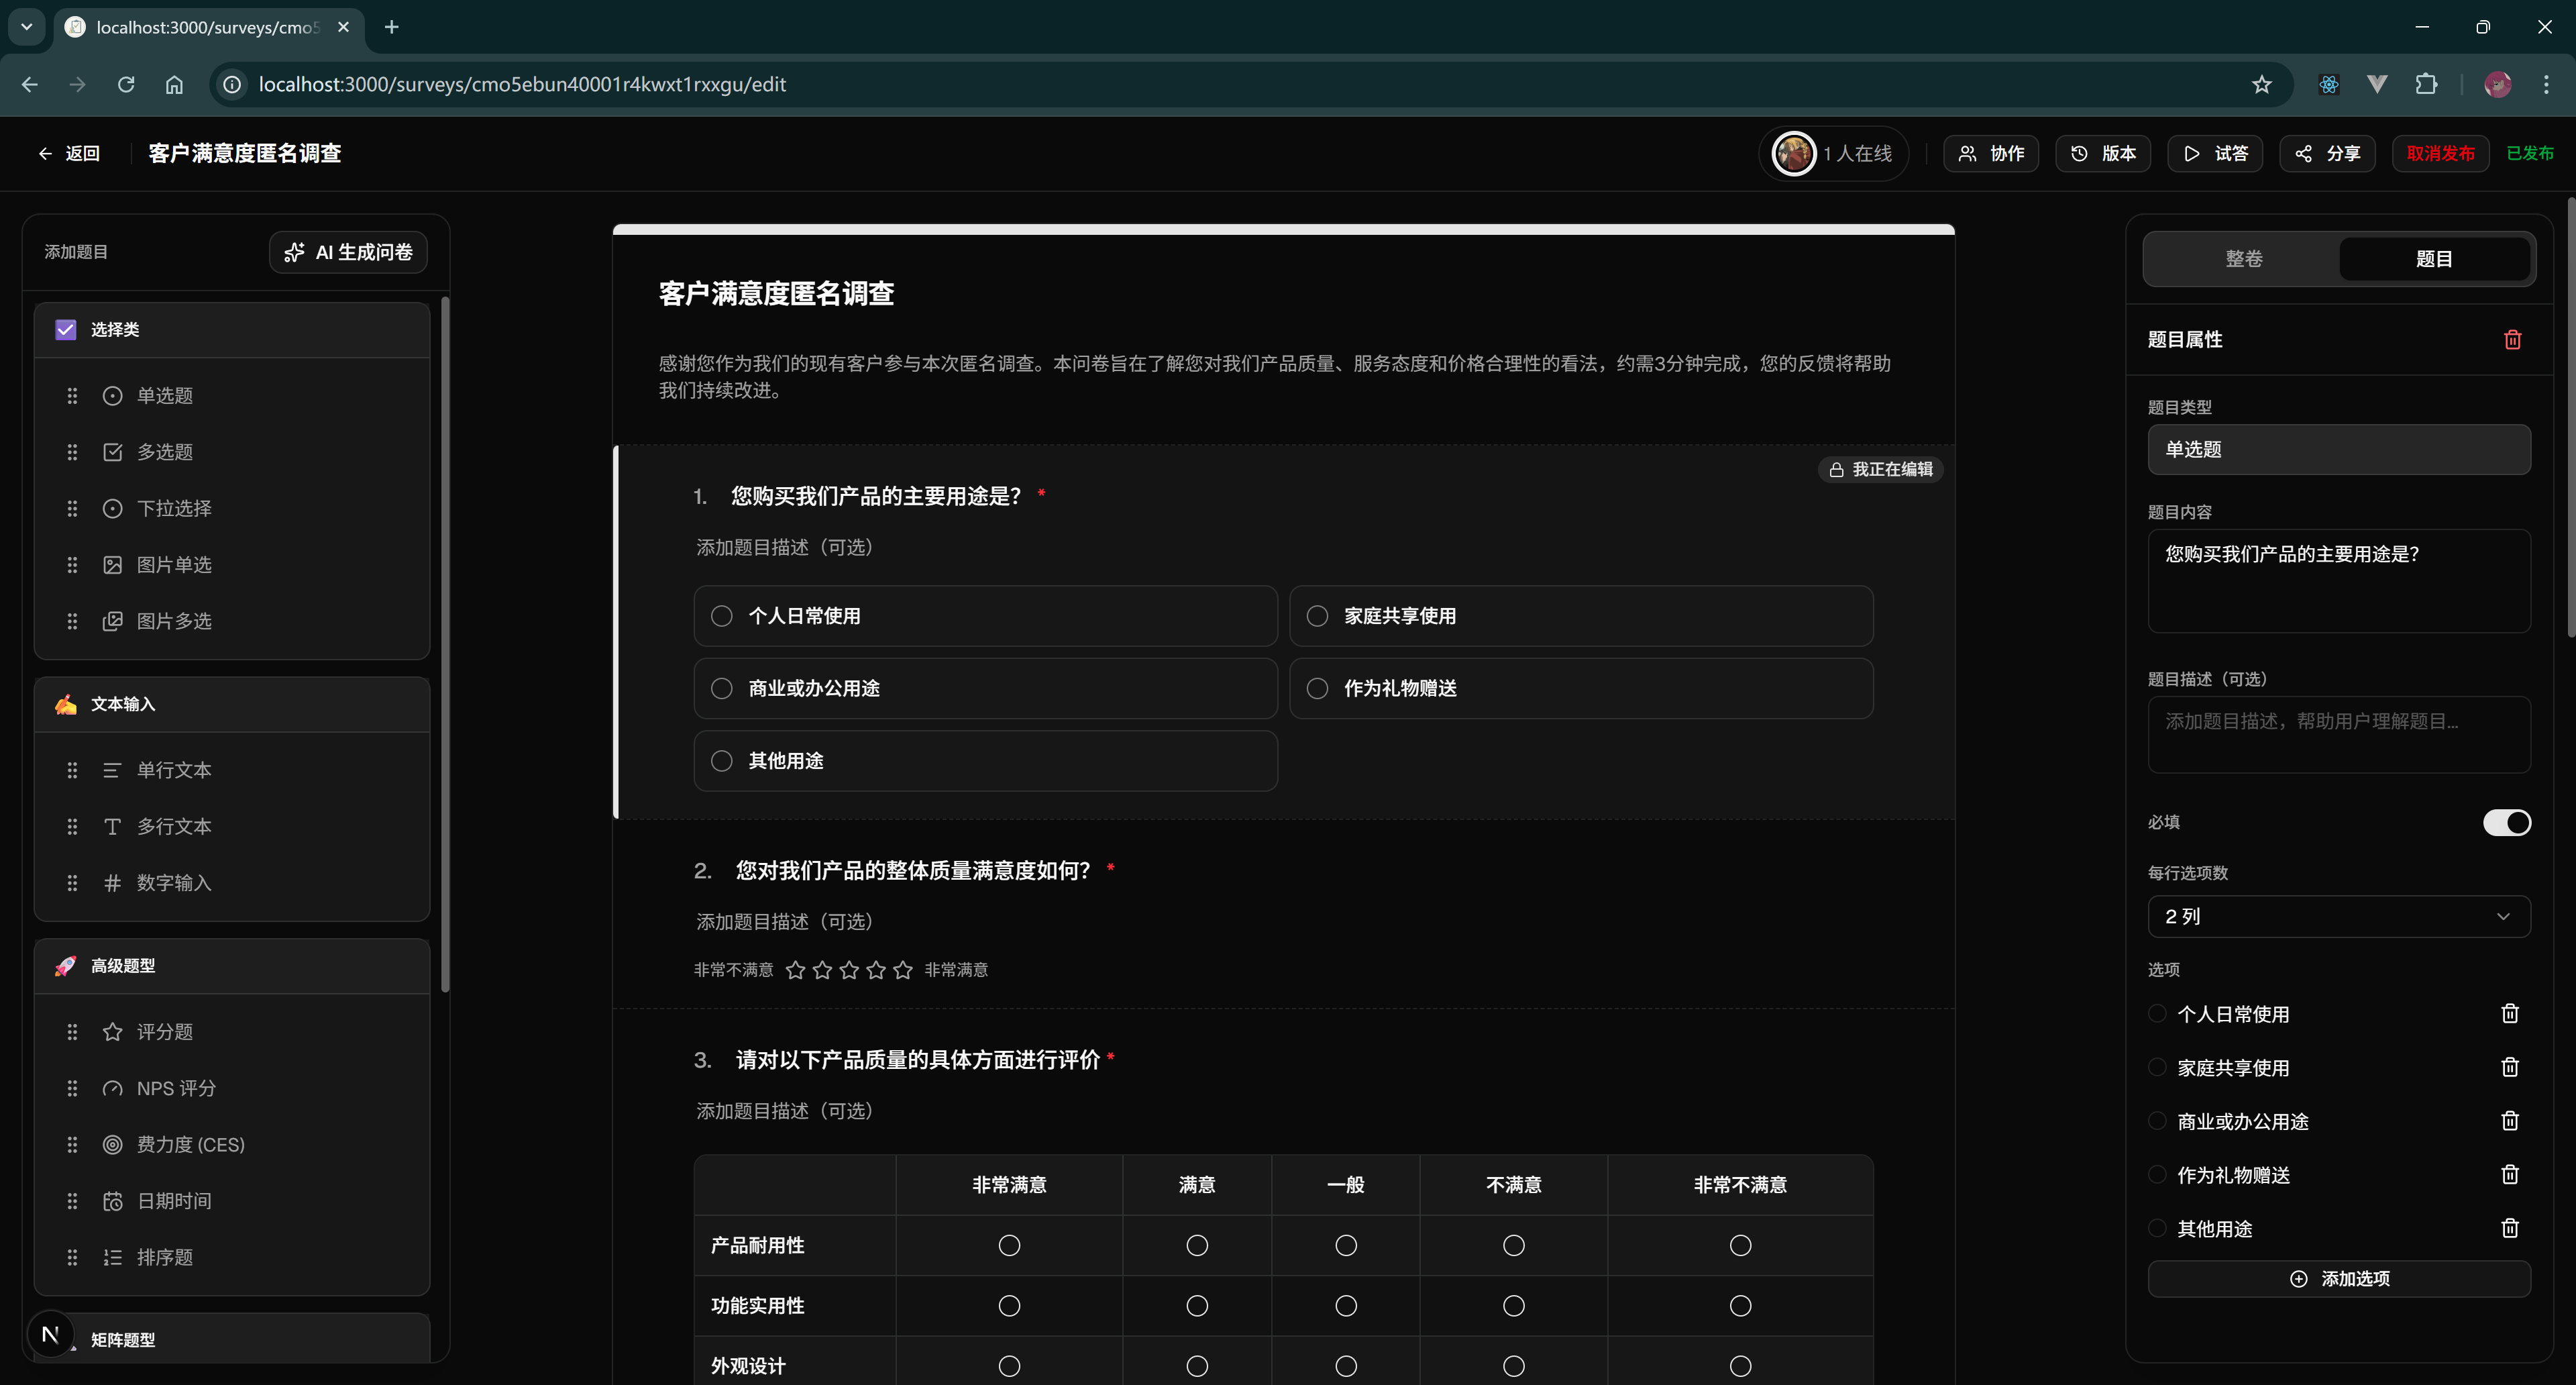
\includegraphics[width=0.95\textwidth]{figures/screenshot-editor.png}
\caption{问卷编辑器三栏布局}
\label{fig:editor-layout}
\end{figure}

\subsubsection{状态管理设计}

编辑器使用 Zustand 管理全局状态。Store 的核心结构如下：

\begin{lstlisting}[language=TypeScript, caption={编辑器 Zustand Store 结构}]
interface EditorState {
  // 问卷基本信息
  survey: Survey | null
  
  // 题目列表
  questions: Question[]
  
  // 当前选中题目
  selectedQuestionId: string | null
  
  // 编辑状态
  isLoading: boolean
  isSaving: boolean
  hasUnsavedChanges: boolean
  
  // Actions
  setSurvey: (survey: Survey) => void
  addQuestion: (type: QuestionType, index?: number) => void
  updateQuestion: (id: string, data: Partial<Question>) => void
  deleteQuestion: (id: string) => void
  reorderQuestions: (from: number, to: number) => void
  selectQuestion: (id: string | null) => void
}
\end{lstlisting}

Zustand 的不可变更新模式确保了 React 组件能够正确响应状态变化。以题目更新为例：

\begin{lstlisting}[language=TypeScript, caption={题目更新 Action 实现}]
updateQuestion: (id, data) => set((state) => ({
  questions: state.questions.map((q) =>
    q.id === id ? { ...q, ...data } : q
  ),
  hasUnsavedChanges: true,
})),
\end{lstlisting}

\subsubsection{题型系统}

系统支持 18 种题型，每种题型由四个核心部分组成：

\begin{enumerate}[label=(\arabic*)]
  \item \textbf{类型定义}：描述题型的数据结构
  \item \textbf{编辑器组件}：在编辑画布中渲染的配置界面
  \item \textbf{预览组件}：答题时的渲染界面
  \item \textbf{统计组件}：结果页中的数据展示
\end{enumerate}

题型通过注册中心统一管理：

\begin{lstlisting}[language=TypeScript, caption={题型注册中心}]
const questionRegistry: Record<QuestionType, QuestionDef> = {
  SINGLE_CHOICE: {
    type: 'SINGLE_CHOICE',
    label: '单选题',
    icon: CircleDot,
    editor: SingleChoiceEditor,
    preview: SingleChoicePreview,
    stats: SingleChoiceStats,
  },
  MULTIPLE_CHOICE: { /* ... */ },
  MATRIX_SINGLE: { /* ... */ },
  // ... 其他题型
}
\end{lstlisting}

\subsubsection{拖拽排序实现}

题目排序采用 HTML5 Drag and Drop API 实现。拖拽过程中需要处理以下事件：

\begin{lstlisting}[language=TypeScript, caption={拖拽排序核心逻辑}]
const handleDragStart = (e: DragEvent, index: number) => {
  e.dataTransfer?.setData('text/plain', String(index))
  setDraggedIndex(index)
}

const handleDrop = (e: DragEvent, targetIndex: number) => {
  const sourceIndex = Number(e.dataTransfer?.getData('text/plain'))
  if (sourceIndex === targetIndex) return
  
  reorderQuestions(sourceIndex, targetIndex)
  
  // 同步到服务器
  fetch(`/api/surveys/${surveyId}/questions/reorder`, {
    method: 'POST',
    body: JSON.stringify({ from: sourceIndex, to: targetIndex }),
  })
}
\end{lstlisting}

\subsubsection{行内编辑高度跳变问题}

在实现题目标题的行内编辑时，遇到了一个典型的 CSS 布局问题。当从预览态（\texttt{div}）切换到编辑态（\texttt{textarea}）时，父容器高度从 36px 跳变为 42.5px。

\textbf{根因分析}：\texttt{textarea} 默认是 \texttt{inline-block} 元素，浏览器会为文字的「降部」（descender）预留基线对齐空间，导致父容器被额外撑开。

\textbf{解决方案}：将 \texttt{textarea} 显式设置为 \texttt{display: block}，彻底脱离行内布局的基线对齐规则。

\begin{lstlisting}[language=CSS, caption={高度跳变问题修复}]
textarea.block {
  display: block;
  width: 100%;
}
\end{lstlisting}

\subsection{问卷发布与版本管理}

\subsubsection{发布流程设计}

问卷发布流程设计如下：

\begin{enumerate}[label=\textbf{\arabic*.}]
  \item 用户在编辑器中完成问卷内容编辑
  \item 点击「发布」按钮，触发版本创建
  \item 系统将当前问卷内容和题目快照保存为新的 \texttt{SurveyVersion} 记录
  \item 生成唯一的 \texttt{shareToken} 作为公开访问标识
  \item 问卷状态更新为已发布
\end{enumerate}

\subsubsection{版本快照机制}

每次发布时，系统将问卷的完整状态序列化为 JSON 存储：

\begin{lstlisting}[language=TypeScript, caption={版本快照创建}]
const version = await prisma.surveyVersion.create({
  data: {
    surveyId,
    version: nextVersionNumber,
    title: survey.title,
    questions: survey.questions.map(q => ({
      id: q.id,
      type: q.type,
      title: q.title,
      required: q.required,
      options: q.options,
      config: q.config,
    })),
  },
})

// 更新问卷的当前版本
await prisma.survey.update({
  where: { id: surveyId },
  data: { currentVersionId: version.id, published: true },
})
\end{lstlisting}

\subsubsection{版本回滚}

版本回滚将问卷内容恢复到指定版本的状态：

\begin{lstlisting}[language=TypeScript, caption={版本回滚实现}]
const rollbackVersion = async (surveyId: string, versionId: string) => {
  const version = await prisma.surveyVersion.findUnique({
    where: { id: versionId },
  })
  
  // 恢复问卷标题
  await prisma.survey.update({
    where: { id: surveyId },
    data: { title: version.title },
  })
  
  // 删除现有题目，重建版本中的题目
  await prisma.question.deleteMany({ where: { surveyId } })
  await prisma.question.createMany({
    data: version.questions.map((q, i) => ({
      surveyId,
      type: q.type,
      title: q.title,
      required: q.required,
      order: i,
      config: q.config,
    })),
  })
}
\end{lstlisting}

\subsubsection{已知问题与处理}

开发过程中发现，问卷列表页的「快速发布」按钮直接切换 \texttt{published} 状态，但未创建 \texttt{SurveyVersion} 记录。这导致用户提交答案时 \texttt{versionId} 为空，触发数据库外键约束错误。

\textbf{当前处理}：隐藏列表页的发布按钮，强制用户通过编辑器中的「版本管理」弹窗进行规范发布。

\textbf{根本修复方向}：统一发布入口，或在 \texttt{publish} API 中自动创建首个版本（如果尚无版本）。

\subsection{问卷填写与提交模块}

\subsubsection{公开问卷访问}

公开问卷通过 \texttt{shareToken} 访问，URL 格式为 \texttt{/s/\{token\}}。系统通过以下流程处理访问请求：

\begin{enumerate}[label=\textbf{\arabic*.}]
  \item 从 URL 中提取 \texttt{shareToken}
  \item 查询对应的问卷和当前版本
  \item 验证问卷是否已发布
  \item 返回问卷数据和题目列表
  \item 记录浏览量（24 小时内同一 IP 去重）
\end{enumerate}

\subsubsection{答案数据结构}

不同题型的答案存储格式不同：

\begin{table}[H]
\centering
\caption{各题型答案存储格式}
\label{tab:answer-formats}
\begin{tabular}{lll}
\toprule
\textbf{题型} & \textbf{存储格式} & \textbf{示例} \\
\midrule
单选题 & 字符串（选项 label） & \texttt{"非常同意"} \\
多选题 & 字符串数组 & \texttt{["选项A", "选项B"]} \\
文本题 & 字符串 & \texttt{"用户输入内容"} \\
评分题 & 数字 & \texttt{4} \\
矩阵单选 & 对象（rowId $\rightarrow$ colId） & \texttt{\{"q1": "col1"\}} \\
GENDER & 字符串（选项 ID） & \texttt{"male"} \\
\bottomrule
\end{tabular}
\end{table}

\subsubsection{提交 API 的 Schema 设计}

提交 API 使用 Zod 进行严格的类型校验。由于答案格式多样，Schema 需要支持多种类型：

\begin{lstlisting}[language=TypeScript, caption={提交 API Zod Schema}]
const submitSchema = z.object({
  answers: z.record(z.string(), z.union([
    z.string(),
    z.array(z.string()),
    z.number(),
    z.null(),
    z.record(z.string(), z.string()), // MATRIX_SINGLE
  ])),
})
\end{lstlisting}

\textbf{矩阵单选题的特殊处理}：矩阵单选题的答案是一个对象（\texttt{\{rowId: colId\}}），因此在 Zod Schema 中需要额外添加 \texttt{z.record(z.string(), z.string())} 类型支持。

\subsubsection{设备与地理位置采集}

系统在提交时自动采集以下信息：

\begin{itemize}
  \item \textbf{设备信息}：通过 User-Agent 解析设备类型、操作系统、浏览器
  \item \textbf{地理位置}：通过 IP 地址解析国家、省份、城市
  \item \textbf{来源渠道}：通过 \texttt{referrer} 或 URL 参数识别
\end{itemize}

地理位置通过 ip-api.com 免费 API 解析。在生产环境（HTTPS）下，由于浏览器安全策略限制，需要通过服务器代理转发请求。

\subsection{结果统计与可视化模块}

\subsubsection{统计页面架构}

结果统计页面采用侧边栏导航 + 内容区的布局，包含五个视图：

\begin{enumerate}[label=(\arabic*)]
  \item \textbf{数据概览}：KPI 卡片、回收趋势、设备/OS 分布、地域分布
  \item \textbf{数据详情}：回答表格、搜索筛选、分页、CSV 导出
  \item \textbf{统计图表}：逐题分析、多种图表类型切换
  \item \textbf{交叉分析}：两题交叉透视表
  \item \textbf{AI 总结}：智能数据分析报告（独立页面）
\end{enumerate}

\subsubsection{逐题统计实现}

逐题统计根据题型选择不同的展示方式：

\begin{lstlisting}[language=TypeScript, caption={逐题统计组件}]
const QuestionStats = ({ question, responses }: Props) => {
  switch (question.type) {
    case 'SINGLE_CHOICE':
    case 'MULTIPLE_CHOICE':
      return <ChoiceStats question={question} responses={responses} />
    case 'RATING':
    case 'NPS':
      return <RatingStats question={question} responses={responses} />
    case 'MATRIX_SINGLE':
      return <MatrixStats question={question} responses={responses} />
    case 'TEXT':
      return <TextStats question={question} responses={responses} />
    default:
      return <GenericStats question={question} responses={responses} />
  }
}
\end{lstlisting}

\subsubsection{GENDER 题型计数逻辑}

统计图表中 GENDER 题型的选项计数曾出现始终为 0 的问题。

\textbf{根因}：大多数选择题的答案存储的是选项 \textbf{label}，而 GENDER 题型特殊，存储的是选项 \textbf{ID}（\texttt{male}/\texttt{female}/\texttt{other}）。统计代码统一使用 \texttt{opt.label} 匹配，导致 GENDER 无法命中。

\textbf{修复}：在统计组件中增加类型判断：

\begin{lstlisting}[language=TypeScript, caption={GENDER 计数修复}]
const matchKey = type === 'GENDER' ? 'id' : 'label'
const count = counts[opt[matchKey]] || 0
\end{lstlisting}

\subsection{AI 辅助模块}

\subsubsection{AI 问卷生成}

AI 问卷生成采用「需求澄清 → 结构化生成」的两阶段流程：

\textbf{阶段一：需求澄清}

系统首先判断用户提供的信息是否足够生成问卷。如果信息不足，返回 1-3 个追问问题：

\begin{lstlisting}[language=TypeScript, caption={需求澄清流程}]
const clarifyResult = await generateObject({
  model: deepseek('deepseek-chat'),
  schema: clarifySchema,
  prompt: `判断以下需求是否足够生成问卷：${userInput}
  如果不足，请提出 1-3 个关键追问。`,
})

if (!clarifyResult.object.isSufficient) {
  return { questions: clarifyResult.object.followUpQuestions }
}
\end{lstlisting}

\textbf{阶段二：结构化生成}

信息充足后，调用 \texttt{generateObject} 生成结构化的问卷数据：

\begin{lstlisting}[language=TypeScript, caption={问卷生成实现}]
const result = await generateObject({
  model: deepseek('deepseek-chat'),
  schema: surveySchema, // Zod Schema 定义问卷结构
  prompt: `根据以下需求生成问卷：${userInput}
  要求：
  - 题目数量适中（5-15题）
  - 题型选择合理
  - 选项覆盖全面`,
})
\end{lstlisting}

\subsubsection{AI 数据总结}

AI 数据总结基于问卷回答数据生成分析报告：

\begin{lstlisting}[language=TypeScript, caption={AI 数据总结流程}]
// 1. 格式化数据为自然语言文本
const formattedData = formatSurveyData(survey, responses)

// 2. 调用 DeepSeek 流式生成
const result = streamText({
  model: deepseek('deepseek-chat'),
  system: '你是一位资深数据分析师...',
  prompt: formattedData,
})

// 3. 返回流式响应
return result.toDataStreamResponse()
\end{lstlisting}

\subsubsection{本地缓存策略}

为避免重复调用 AI API，系统实现了本地缓存：

\begin{lstlisting}[language=TypeScript, caption={AI 总结缓存实现}]
const useSummaryCache = (surveyId: string) => {
  const key = `ai-summary:${surveyId}`
  
  const get = () => {
    const raw = localStorage.getItem(key)
    if (!raw) return null
    const cached = JSON.parse(raw)
    // 当回答数变化时自动失效
    if (cached.totalResponses !== currentTotal) return null
    return cached.content
  }
  
  const set = (content: string, totalResponses: number) => {
    localStorage.setItem(key, JSON.stringify({
      content, totalResponses, timestamp: Date.now()
    }))
  }
  
  return { get, set }
}
\end{lstlisting}

\textbf{当前状态}：AI 总结页面功能完整，但鉴于数据量较小时生成质量不稳定，已暂时从侧边栏隐藏入口，保留页面代码供后续优化。

\subsection{实时协作模块}

\subsubsection{协作架构}

实时协作基于 Pusher 的 Presence Channel 实现。每个问卷对应一个独立的 Presence Channel，频道名格式为 \texttt{presence-survey-\{surveyId\}}。

\begin{figure}[H]
\centering
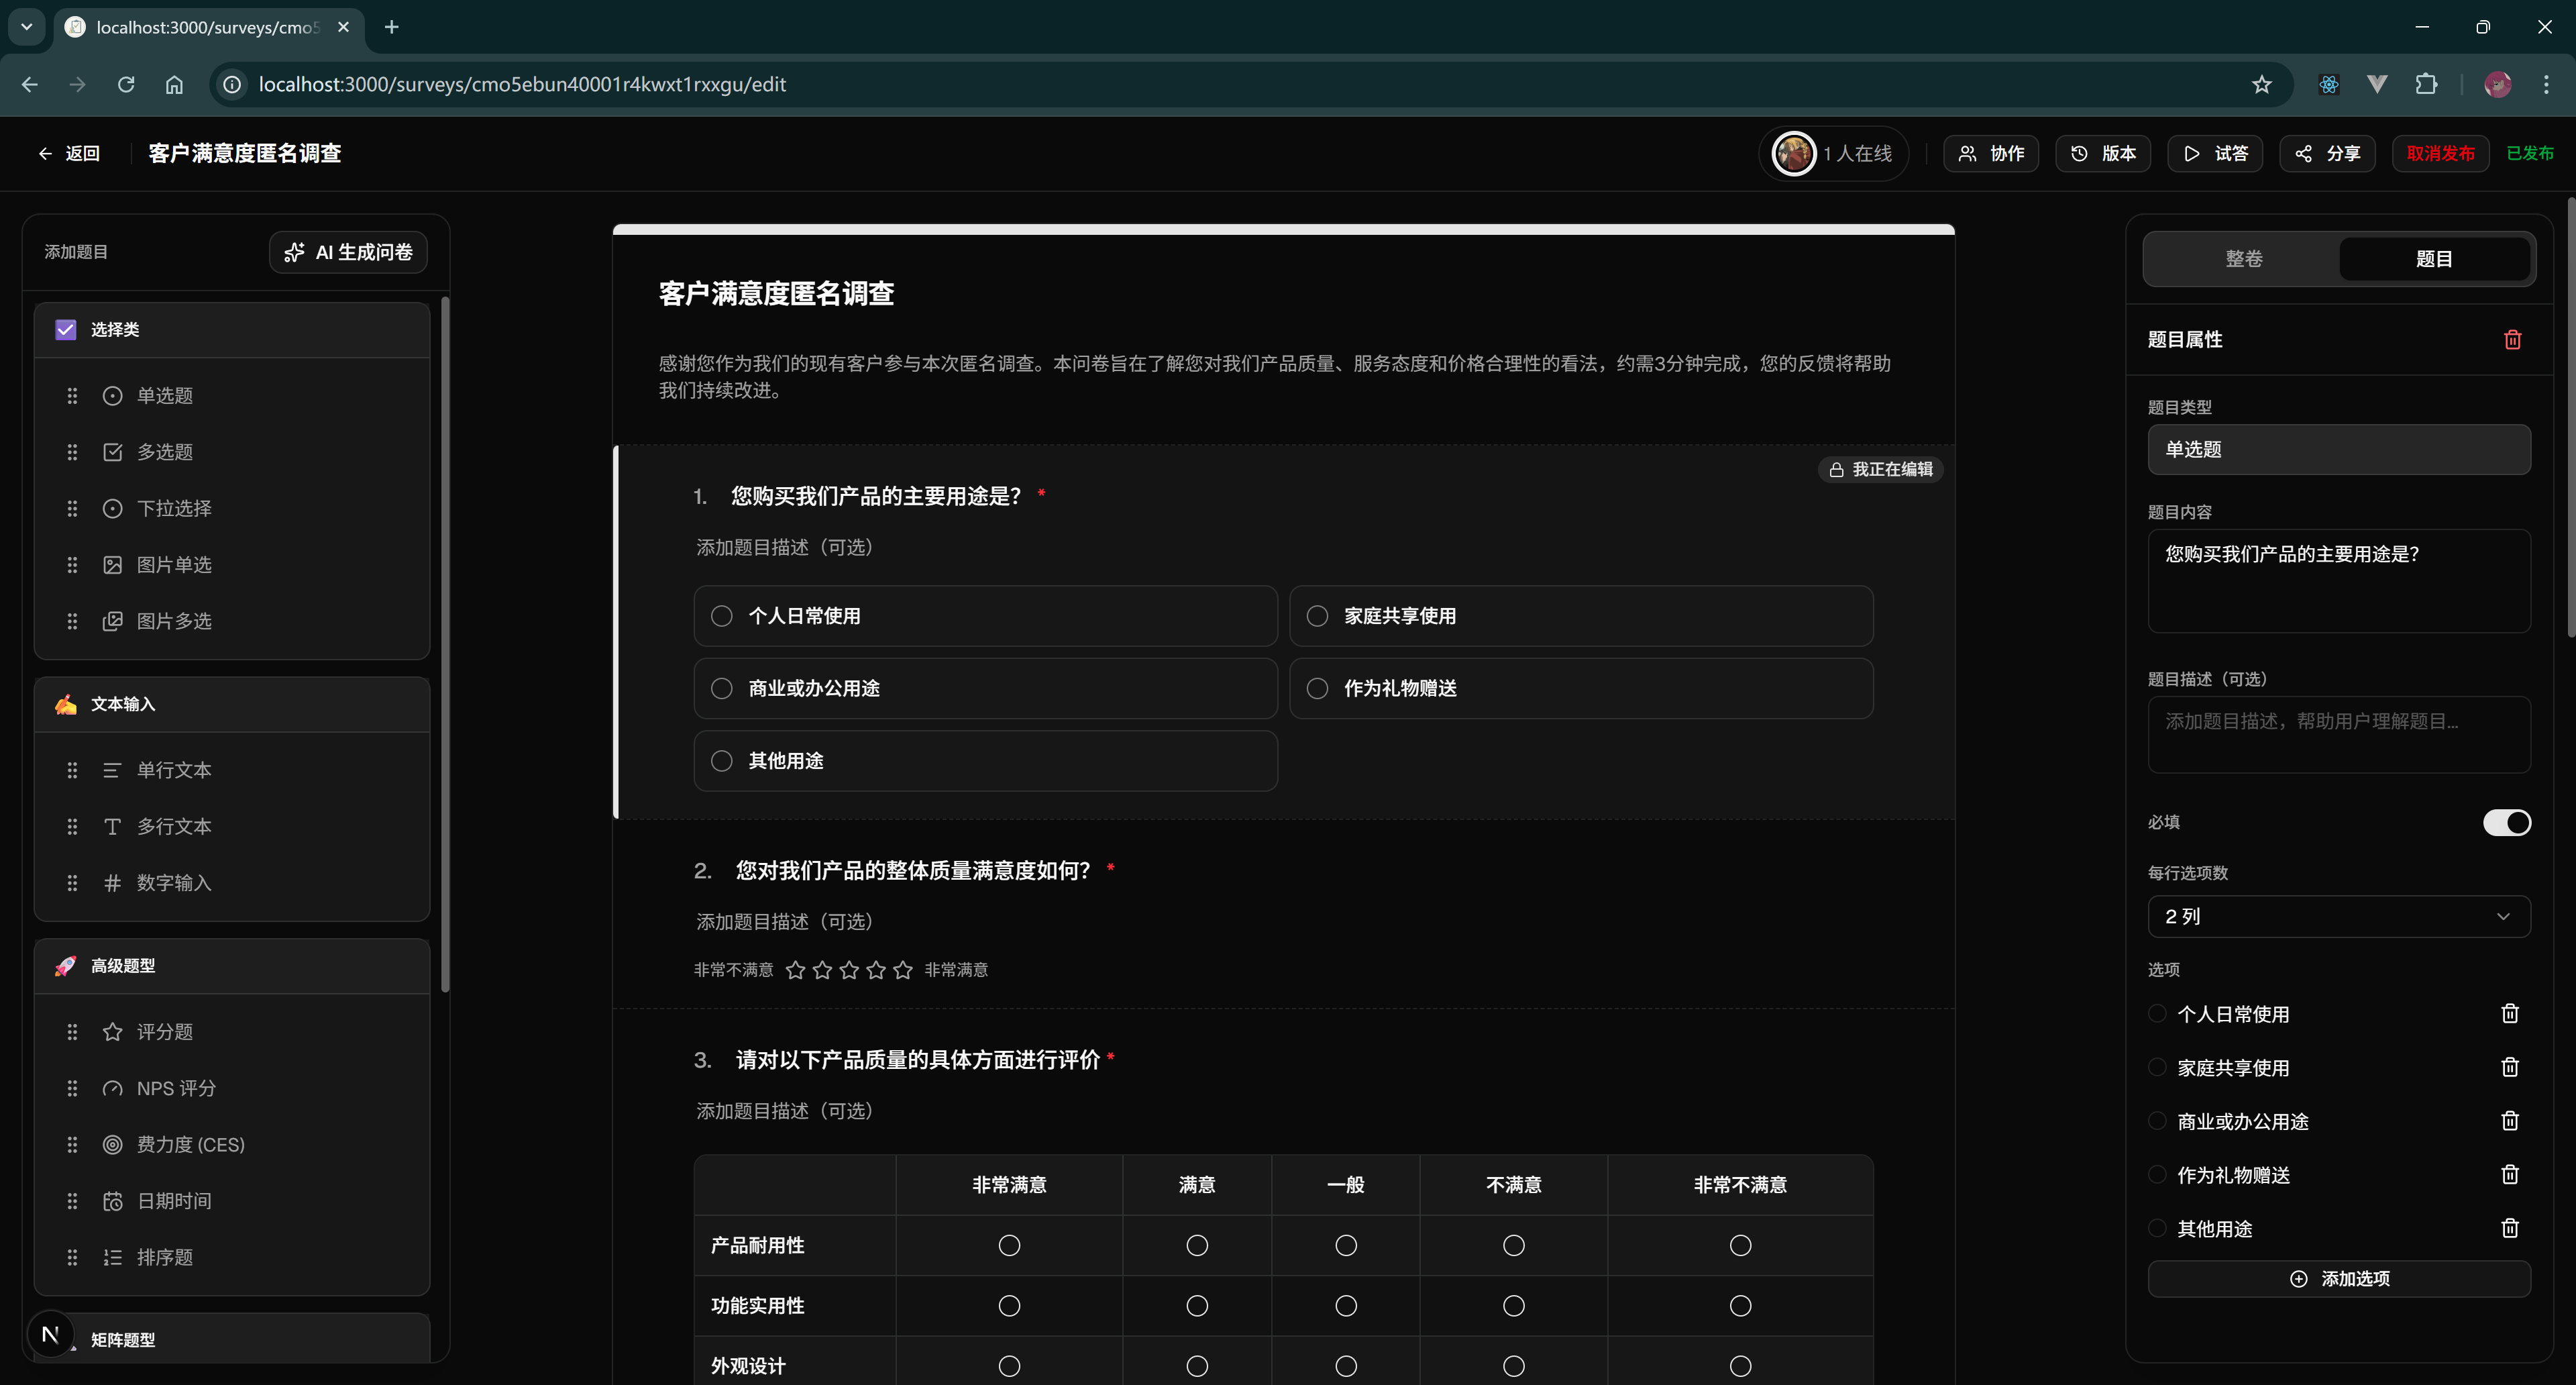
\includegraphics[width=0.95\textwidth]{figures/screenshot-editor.png}
\caption{实时协作编辑界面}
\label{fig:collaboration-arch}
\end{figure}

\subsubsection{题目乐观锁定}

为防止多人同时编辑同一题目，系统实现了题目级的乐观锁定：

\begin{lstlisting}[language=TypeScript, caption={题目锁定机制}]
// 选中题目时发送锁定请求
const lockQuestion = async (questionId: string) => {
  await fetch('/api/surveys/collaboration/lock', {
    method: 'POST',
    body: JSON.stringify({ surveyId, questionId }),
  })
  
  // 广播锁定事件
  channel.trigger('client-question-locked', {
    questionId,
    userId: currentUser.id,
    userName: currentUser.name,
  })
}

// 切换题目时释放锁定
const unlockQuestion = async (questionId: string) => {
  await fetch('/api/surveys/collaboration/unlock', {
    method: 'POST',
    body: JSON.stringify({ surveyId, questionId }),
  })
}
\end{lstlisting}

\subsubsection{实时同步事件}

系统通过以下事件实现状态同步：

\begin{table}[H]
\centering
\caption{Pusher 事件定义}
\label{tab:pusher-events}
\begin{tabular}{lll}
\toprule
\textbf{事件名} & \textbf{方向} & \textbf{说明} \\
\midrule
\texttt{question-locked} & client $\rightarrow$ client & 题目被锁定 \\
\texttt{question-unlocked} & client $\rightarrow$ client & 题目解锁 \\
\texttt{question-added} & client $\rightarrow$ client & 新增题目 \\
\texttt{question-updated} & client $\rightarrow$ client & 题目内容更新 \\
\texttt{question-deleted} & client $\rightarrow$ client & 删除题目 \\
\texttt{questions-reordered} & client $\rightarrow$ client & 题目重排 \\
\texttt{survey-updated} & client $\rightarrow$ client & 问卷信息更新 \\
\bottomrule
\end{tabular}
\end{table}

\subsubsection{异常处理}

系统处理了以下协作异常场景：

\begin{itemize}
  \item \textbf{成员意外离开}：通过 Presence Channel 的 \texttt{member-removed} 事件检测，自动释放该成员锁定的所有题目
  \item \textbf{网络断开重连}：Pusher 自动处理重连，恢复频道订阅
  \item \textbf{并发编辑冲突}：乐观锁定机制确保同一时刻只有一个用户编辑特定题目
\end{itemize}

\begin{lstlisting}[language=TypeScript, caption={成员离开自动解锁}]
channel.bind('pusher:member_removed', (member) => {
  // 释放该成员锁定的所有题目
  fetch('/api/surveys/collaboration/unlock-all', {
    method: 'POST',
    body: JSON.stringify({ surveyId, userId: member.id }),
  })
})
\end{lstlisting}
